% Author: Simon-Pierre Boucher — contact@spboucher.ai
%
% ═══════════════════════════════════════════════════════════════════════
% APPENDICES
% ═══════════════════════════════════════════════════════════════════════
\appendix

\section{Additional Figures}
\label{app:figures}

\begin{figure}[H]
    \centering
    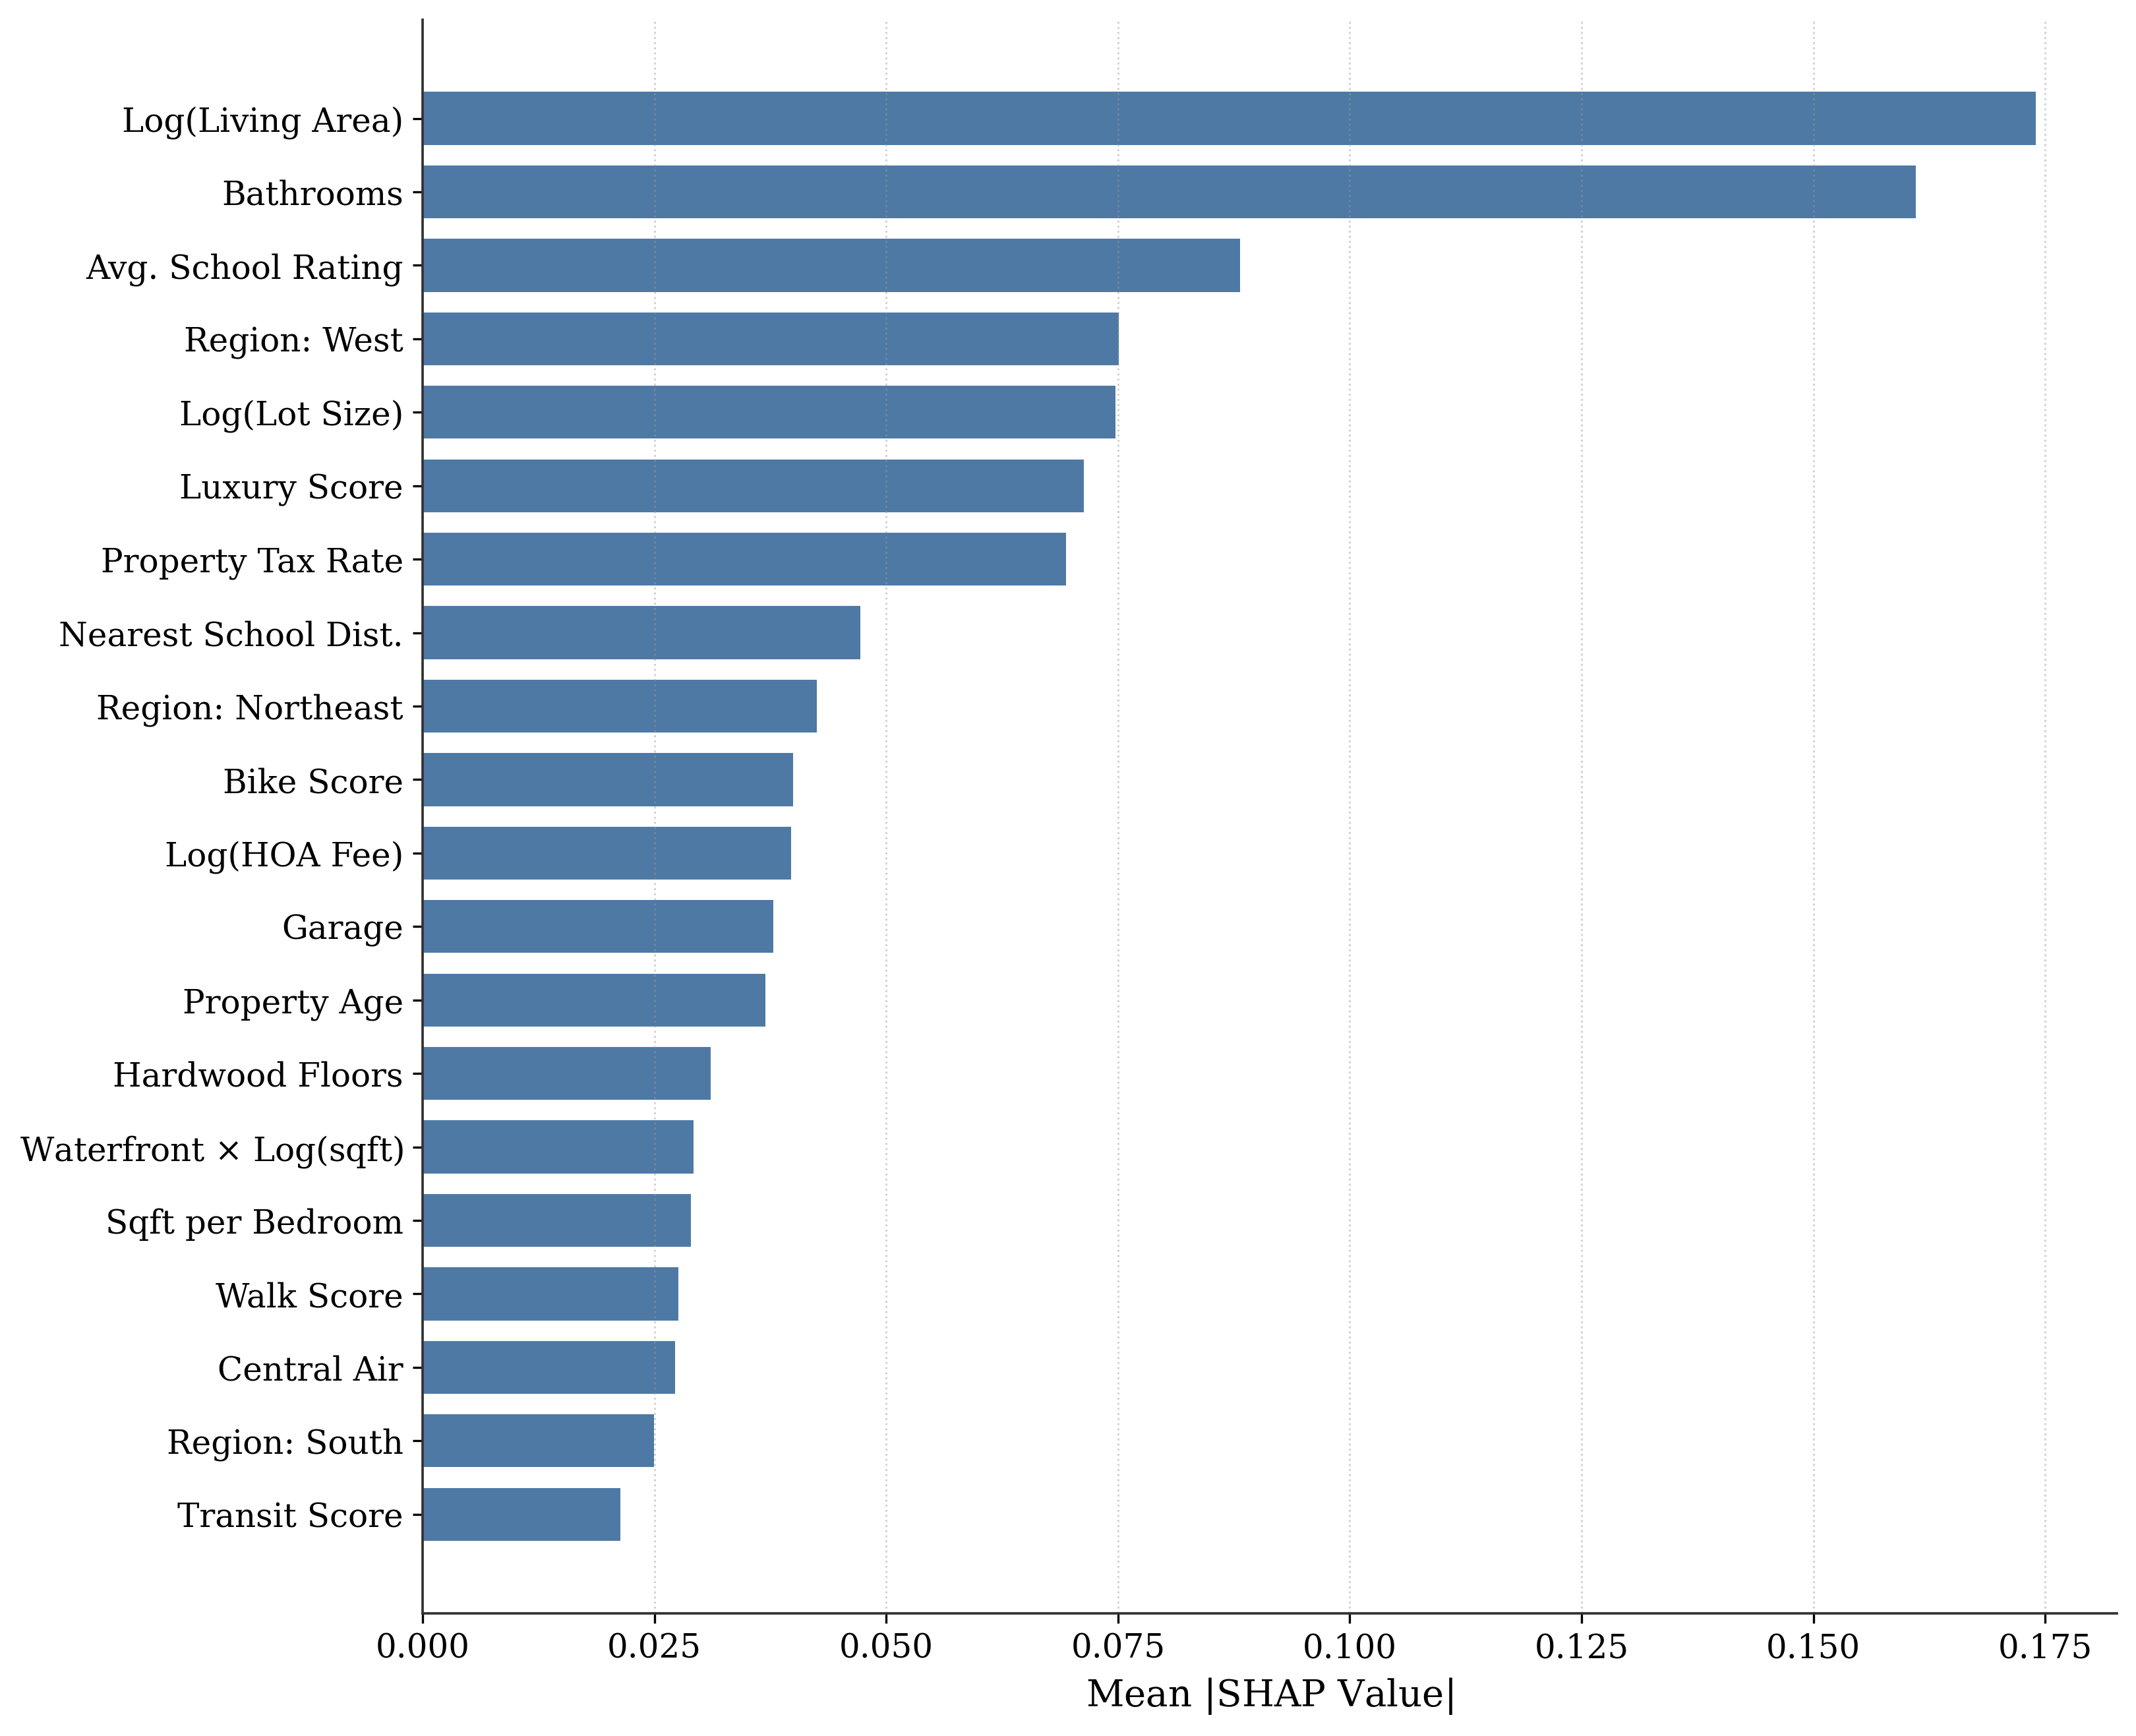
\includegraphics[width=0.85\textwidth]{figures/fig6_shap_importance.png}
    \caption{Feature Importance Bar Chart: Mean Absolute SHAP Values (XGBoost). These values reflect predictive contributions, not causal importance.}
    \label{fig:shap_bar}
\end{figure}

\begin{figure}[H]
    \centering
    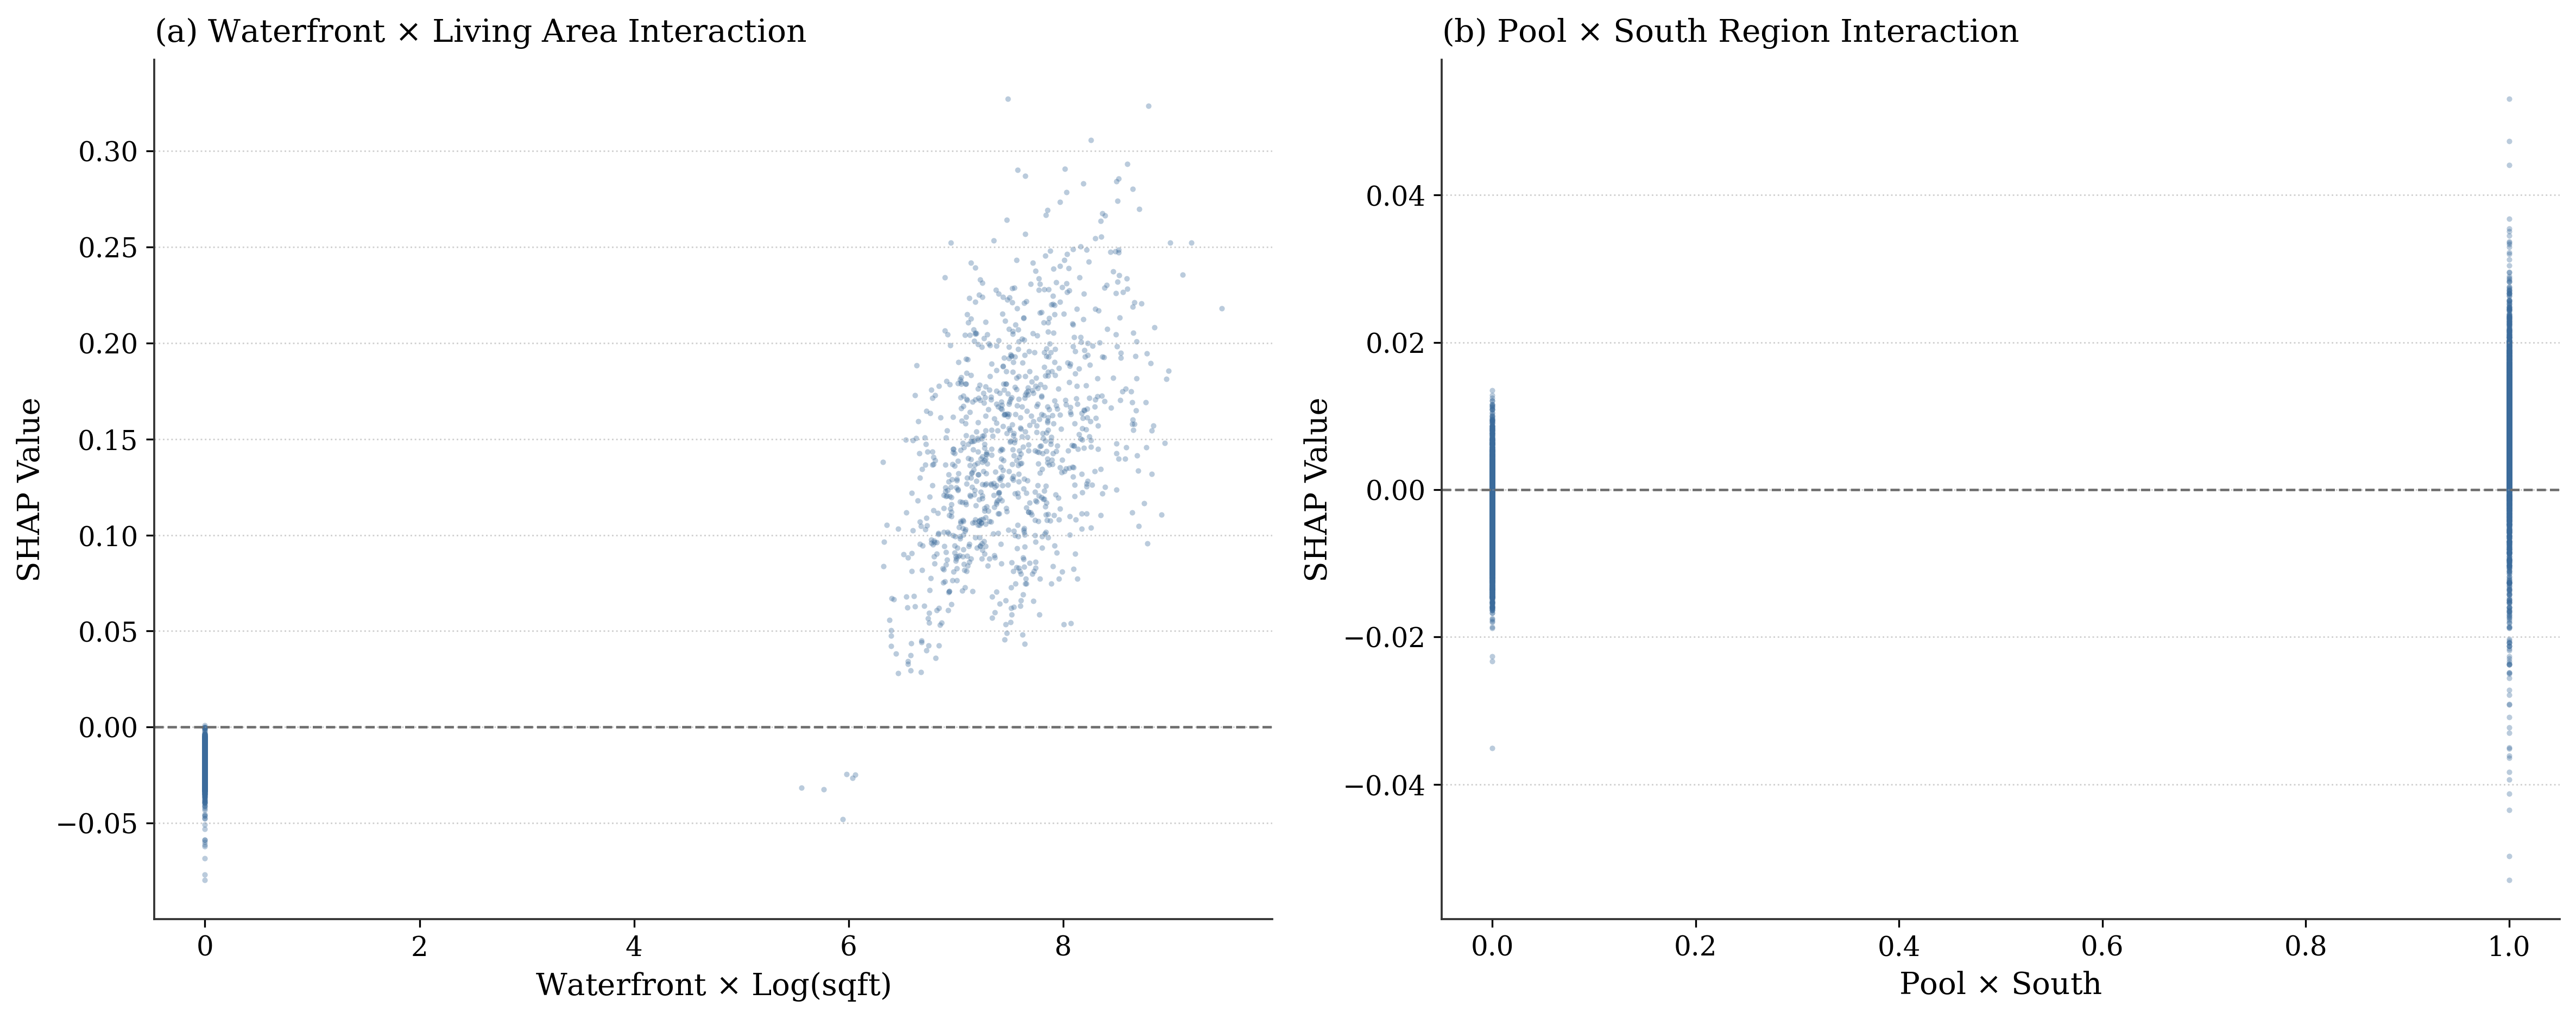
\includegraphics[width=\textwidth]{figures/fig11_shap_interactions.png}
    \caption{SHAP Values for Interaction Terms: (a) Waterfront $\times$ Log(Living Area); (b) Pool $\times$ South Region}
    \label{fig:shap_interactions}
\end{figure}


\section{Full OLS Coefficient Table}
\label{app:ols_full}

Table~\ref{tab:ols_full} reports the complete set of standardized OLS coefficients, including all categorical controls.

\begin{landscape}
\begin{table}[H]
\centering
\caption{Full OLS Regression Results Including All Categorical Controls (Standardized)}
\label{tab:ols_full}
\begin{threeparttable}
\scriptsize
\renewcommand{\arraystretch}{0.9}
\begin{tabular}{lrrlclrrl}
\toprule
Variable & Coeff. & SE & Sig. & & Variable & Coeff. & SE & Sig. \\
\midrule
Constant & 12.510 & 0.010 & *** & & Roof: Metal & 0.070 & 0.008 & *** \\
$\ln$(Living Area)$^\dagger$ & 0.312 & 0.003 & *** & & Roof: Shingle/Comp & $-$0.074 & 0.008 & *** \\
Bedrooms$^\dagger$ & $-$0.068 & 0.002 & *** & & Roof: Tile & $-$0.110 & 0.008 & *** \\
Bathrooms$^\dagger$ & 0.236 & 0.003 & *** & & Roof: Slate & 0.008 & 0.017 & \\
Age$^\dagger$ & $-$0.042 & 0.014 & ** & & Roof: Other & 0.033 & 0.008 & *** \\
Age$^{2\dagger}$ & 0.051 & 0.002 & *** & & Roof: Unknown & 0.004 & 0.008 & \\
Stories$^\dagger$ & 0.000 & 0.000 & & & Constr: Concrete/Block & 0.269 & 0.003 & *** \\
Bath/Bed Ratio$^\dagger$ & $-$0.021 & 0.002 & *** & & Constr: Stucco & 0.149 & 0.002 & *** \\
Sqft/Bed$^\dagger$ & $-$0.002 & 0.002 & & & Constr: Stone & 0.145 & 0.005 & *** \\
$\ln$(Lot Size)$^\dagger$ & 0.070 & 0.001 & *** & & Constr: Wood/Frame & 0.103 & 0.002 & *** \\
Pool & 0.029 & 0.003 & *** & & Constr: Vinyl & 0.012 & 0.002 & *** \\
Spa & 0.033 & 0.003 & *** & & Constr: Steel & 0.027 & 0.014 & * \\
Basement & $-$0.042 & 0.002 & *** & & Constr: Other & 0.075 & 0.002 & *** \\
Fireplace & $-$0.002 & 0.002 & & & Constr: Unknown & 0.177 & 0.002 & *** \\
Garage & 0.109 & 0.002 & *** & & Found: Concrete & 0.217 & 0.005 & *** \\
Waterfront & $-$0.135 & 0.032 & *** & & Found: Crawlspace & 0.181 & 0.006 & *** \\
Central Air & 0.069 & 0.001 & *** & & Found: Slab & 0.122 & 0.005 & *** \\
Forced Air & $-$0.023 & 0.002 & *** & & Found: Pier/Raised & 0.161 & 0.006 & *** \\
Hardwood & 0.125 & 0.001 & *** & & Found: Stone & 0.032 & 0.010 & ** \\
Parking$^\dagger$ & 0.000 & 0.099 & & & Found: Other & 0.144 & 0.006 & *** \\
Luxury$^\dagger$ & 0.044 & 0.002 & *** & & Found: Unknown & 0.174 & 0.005 & *** \\
Walk$^\dagger$ & $-$0.011 & 0.001 & *** & & Northeast & 0.487 & 0.003 & *** \\
Bike$^\dagger$ & 0.072 & 0.001 & *** & & South & 0.022 & 0.003 & *** \\
Transit$^\dagger$ & 0.052 & 0.001 & *** & & West & 0.401 & 0.003 & *** \\
School Rating$^\dagger$ & $-$0.049 & 0.001 & *** & & sqft$\times$Age$^\dagger$ & $-$0.110 & 0.014 & *** \\
School Count$^\dagger$ & $-$0.002 & 0.001 & *** & & Pool$\times$South & 0.008 & 0.001 & *** \\
School Dist.$^\dagger$ & $-$0.016 & 0.001 & *** & & WF$\times$sqft$^\dagger$ & 0.137 & 0.009 & *** \\
Tax Rate$^\dagger$ & $-$0.029 & 0.001 & *** & & Base$\times$North & $-$0.025 & 0.001 & *** \\
Condo & $-$0.037 & 0.004 & *** & & Condo$\times$Walk$^\dagger$ & 0.082 & 0.001 & *** \\
HOA & $-$0.108 & 0.002 & *** & & Age$\times$Lux$^\dagger$ & 0.044 & 0.001 & *** \\
$\ln$(HOA+1)$^\dagger$ & 0.044 & 0.001 & *** & & & & & \\
New Constr. & 0.103 & 0.003 & *** & & & & & \\
Foreclosure & $-$0.406 & 0.010 & *** & & & & & \\
\midrule
\multicolumn{9}{l}{$R^2 = 0.634$, Adj.\ $R^2 = 0.634$, $N = 788{,}842$, $F = 18{,}712.5$, RMSE $= 0.489$} \\
\bottomrule
\end{tabular}
\begin{tablenotes}
\footnotesize
\item \textit{Notes:} HC3 robust standard errors. $^\dagger$Standardized continuous variables. Reference categories: Roof = Flat; Construction = Brick; Foundation = Basement; Region = Midwest. *** $p<0.001$, ** $p<0.01$, * $p<0.05$.
\end{tablenotes}
\end{threeparttable}
\end{table}
\end{landscape}


\section{Robustness Agenda}
\label{app:robustness_agenda}

The following robustness checks and extensions are planned or completed. Items marked with $\checkmark$ have been completed in this version; unmarked items are left for future work.

\begin{enumerate}[nosep]
    \item[$\checkmark$] ZIP3-level fixed effects (Section~\ref{sec:progressive_fe}).
    \item County-level and MSA-level fixed effects.
    \item Spatial lag and spatial error model estimation.
    \item Spatial cross-validation (train on some regions, test on others) at finer geographic levels.
    \item[$\checkmark$] Inter-quantile Wald tests for coefficient equality across quantiles (Section~\ref{sec:qr_results}).
    \item[$\checkmark$] Re-estimation excluding imputed observations (Section~\ref{sec:imputation_sensitivity}).
    \item CatBoost benchmark with native categorical handling.
    \item Nested cross-validation for hyperparameter tuning.
    \item[$\checkmark$] SHAP stability comparison across XGBoost, LightGBM, and Random Forest (Section~\ref{sec:shap_results}).
    \item Integration of climate risk data from First Street Foundation or FEMA flood maps.
    \item Replication using transaction prices from recently sold listings.
    \item GAM/spline models to decompose the ML gain into non-linearity versus spatial partitioning.
    \item Comparison of sample distribution to ACS and Census benchmarks by state and price tier.
    \item Calibration plots by price decile for all models.
    \item[$\checkmark$] Winsorization sensitivity (Section~\ref{sec:winsorization}).
    \item[$\checkmark$] Feature ablation analysis for XGBoost (Section~\ref{sec:ablation}).
    \item[$\checkmark$] XGBoost with latitude/longitude coordinates (Section~\ref{sec:geo_features}).
    \item[$\checkmark$] XGBoost without geographic features (Section~\ref{sec:geo_features}).
    \item[$\checkmark$] Moran's $I$ subsample stability (Section~\ref{sec:spatial_autocorrelation}).
    \item[$\checkmark$] Quantile regression stability across 10 subsamples (Section~\ref{sec:qr_stability}).
\end{enumerate}


\section{Reproducibility Checklist}
\label{app:reproducibility}

\begin{table}[H]
\centering
\caption{Reproducibility Checklist}
\label{tab:reproducibility}
\begin{threeparttable}
\small
\begin{tabular}{p{6cm}p{3cm}p{4cm}}
\toprule
Item & Status & Notes \\
\midrule
\multicolumn{3}{l}{\textit{Data}} \\
Data source identified & Yes & Zillow active listings \\
Sample construction documented & Yes & Table~\ref{tab:attrition} \\
Missing data rates reported & Yes & Table~\ref{tab:missing} \\
Imputation method documented & Yes & State-level medians \\
Imputation sensitivity tested & Yes & Table~\ref{tab:imputation} \\
\midrule
\multicolumn{3}{l}{\textit{Methodology}} \\
Model specifications documented & Yes & Eq.~\ref{eq:ols}--\ref{eq:moran} \\
Hyperparameters reported & Yes & Section~\ref{sec:methodology} \\
Random seeds reported & Yes & Seed = 42 \\
Validation design documented & Yes & Section~\ref{sec:validation_designs} \\
\midrule
\multicolumn{3}{l}{\textit{Results}} \\
Point estimates reported & Yes & Tables~\ref{tab:ols_results}--\ref{tab:shap_stability} \\
Standard errors / CIs reported & Yes (OLS, QR) & HC3 standard errors \\
Multiple comparisons addressed & Partially & Inter-quantile tests \\
Effect sizes in natural units & Yes & Table~\ref{tab:ols_unstd} \\
\midrule
\multicolumn{3}{l}{\textit{Robustness}} \\
Sensitivity to data quality & Yes & Sections~\ref{sec:imputation_sensitivity}--\ref{sec:winsorization} \\
Sensitivity to model choice & Yes & Table~\ref{tab:ml_comparison} \\
Sensitivity to validation design & Yes & Tables~\ref{tab:geo_holdout}--\ref{tab:geo_role} \\
Cross-model stability & Yes & Table~\ref{tab:shap_stability} \\
\midrule
\multicolumn{3}{l}{\textit{Code and Data Availability}} \\
Code available & Yes & Replication package (\texttt{src/}, \texttt{scripts/}, pinned \texttt{requirements.txt}) \\
Data available & On request & Subject to Zillow ToS \\
\bottomrule
\end{tabular}
\begin{tablenotes}
\small
\item \textit{Notes:} This checklist follows recommended practices for empirical reproducibility in applied economics.
\end{tablenotes}
\end{threeparttable}
\end{table}
